Im vorherigen Kapitel, dem Retargeting Schritt \nameref{ch:Content2:sec:Retargeting},
wird eine vorberechnete Retargeting-Textur verwendet. Diese speichert eine
Permutation, die unsere blue noise Textur vom frame t in eine
blue noise Textur vom frame t+1 umwandelt. Diese Permutation wird 
dann auf die Startwerte angewandt bevor das nächste frame t+1 gerendert wird.
Dadurch werden die blue noise Umverteilung der Sorting Phase \nameref{ch:Content2:sec:Sorting}
akkumuliert und die optische Aufwertung erst richtig sichtbar.
Die retarget Textur wird mit Hilfe von \textbf{simulated annealing} 
\cite{hal02158423} berechnet. Wir wollen somit eine approximativ 
optimale Lösung finden: Permutiere Pixel der blue noise Textur von 
frame t bis Sie sehr ähnlich verteilt sind wie die Pixel der blue noise
Textur von frame t+1. Dabei ist die Lokalität der Vertauschungen, 
welche wir bereits in der Sorting Phase\nameref{ch:Content2:sec:Sorting}
verwendet haben, wichtig.

Die Funktion nach der optimiert wird ist an die Formel aus\cite{georgiev2016blue} angelehnt.
\begin{equation}\label{eq:pixel energy function}
    E(M) = \sum_{p \neq q}E(p,q) = 
           \sum_{p \neq q} \mathrm{e}^{-\frac{\Vert{p_{i}-q_{i}}\Vert^{2}}{\sigma_{i}^{2}} -
           \frac{\Vert{p_{s}-q_{s}}\Vert^{d/2}}{\sigma_{s}^{2}}}
\end{equation}
Wähle nach \cite{ulichney1993void} $\sigma_{i} = 2.1$ und $\sigma_{s} = 1$ 
Zu den Pixeln p,q beschreibt $p_{i}$ und $q_{i}$ ihre jeweiligen Koordinaten.
Und $p_{s}$ und $q_{s}$ sind ihre d-dimensionalen Samplewerte.


\begin{algorithm}[H]
    \caption{\textbf{Simulated Annealing} finde sehr gute Lösung}
    \begin{algorithmic}[1]
        \State initialisiere Startzustand $s=s_{0}$
        \For{i=1...maxSteps}
        \State //Radius für Nachbarschaftssuche ist auf 6 festgesetzt
        \State $s_{neu}\leftarrow$Nachbarzustand(s)
        \If{P(Energie(s), Energie($s_{new}$))$\ge$ random(0,1)} 
        \State s = $s_{new}$
        \EndIf
        \EndFor
        \State return Endzustand s;
    \end{algorithmic}
    \label{alg:retargeting}
\end{algorithm}

Als Startzustand $s_{0}$ definieren wir eine Permutation, die alle 
Elemente auf sich selbst abbildet.
Um von einem Zustand s zu einem neuem Zustand $s_{new}$ zu kommen,
definieren wir eine Nachbarschaftsfunktion \textit{Nachbarzustand()}. 
Diese kann zwei Elemente genau dann vertauschen, wenn Sie in einem 
gegenseitigen Radius r = 6 erreichbar sind. Dabei vertauschen wir
in jedem Schritt ein Pixelpaar. 
Die Wahrscheinlichkeitsfunktion zur neuen Zustandsannahme
P(Energie(s), Energie($s_{new}$)) beschreibt, ob wir den neu
gewählten Zustand $s_{new}$ übernehmen. Dabei wird klassischerweise die
Akzeptanz von Zuständen mit höherer Energie immer kleiner.(bzw. die 
Toleranz gegenüber größeren Fehlern im Bezug zur Zeit). Die allgemeine Akzeptanz von 
Zuständen mit höherer Energie ist dabei von fundamentaler Bedeutung.
Somit verlassen wir möglicherweiße nur lokale Maxima.
Die zu minimierende Energiefunktion E\nameref{eq:pixel energy function} betrachtet
dabei zwei 

\begin{figure}[H]\label{pic:Retargeting}
    \centering
    \begin{minipage}[t]{0.45\linewidth}
        \centering
        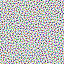
\includegraphics[width=\linewidth]{content/simulatedAnnealing/Bilder/LDR_RGBA_64.png}
        \caption{Blue noise Textur 64x64}
    \end{minipage}
    \hfill
    \begin{minipage}[t]{0.45\linewidth}
        \centering
        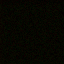
\includegraphics[width=\linewidth]{content/simulatedAnnealing/Bilder/LDR_RGBA_64_retarget_texture.png}
        \caption{Permutation; gespeichert in R,G-Channel einer .png}
    \end{minipage}
\end{figure}

